% !TEX root = ../my-thesis.tex
%
\chapter{Data Analysis}
\label{sec:analysis}
In this chapter the models calculated for each country are reviewed. First, a look at the standardised incidence rate for each country is taken, before spatial models, spatio-temporal models and finally predictive models are discussed.
\section{Standardised Incidence Ratio}
This section takes a brief look at the standardised incidence ratio for the countries of interest.
\subsection{Standardised Incidence Ratio for Germany}
When looking at the standardised incidence ratio for Germany, it is noticeable that the actual number of infections in the eastern parts of Germany, especially in Saxony, is considerably higher than the expected number of infections. Furthermore, parts of Bavaria have an increased standardised incidence ratio compared to the rest of Germany, excluding Saxony. This could be due to the fact that the regions share a border with the Czech Republic, a country that is substantially more affected by Covid-19 than Germany. The northern parts of Germany show the lowest SIR which is possibly due to the fact that this region is sparsely populated. For more information, see Figure~\ref{sirgermany}.
% \begin{figure}[H]
%   \centering
%   \includesvg[width = 1.2\textwidth]{sir_germany.svg}
%   \caption{The standardised incidence ratio for Germany based on the data of the 24th of March 2021}
%   \label{sirgermany}
% \end{figure}
\begin{figure}[H]
  \centering
  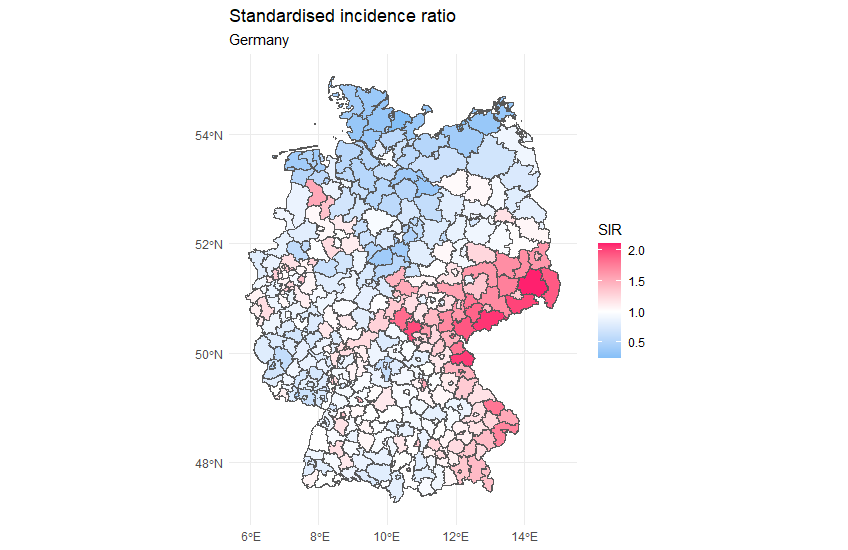
\includegraphics[width = 1.2\textwidth]{sir_germany.png}
  \caption{The standardised incidence ratio for Germany based on the data of the 24th of March 2021}
  \label{sirgermany}
\end{figure}
\subsection{Standardised Incidence Ratio for Norway}
Looking at the standardised incidence rate for Norway, a standardised incidence rate of less than 1 can be seen for most municipalities north of Trondheim. In the southern parts of Norway there are several municipalities with a rate above 1, for example the standardised incidence rate around the capital Oslo is around 2. However, the two small municipalities, Hyllestad and Ulvik, have the highest standardised incidence rate in Norway. In Hyllestad, 95 of 1328 people have been infected with Covid-19 so far, while in Ulvik, 134 of 1080 people have been infected so far. \\
The SIR in Hyllestad is around 4.5, following an outbreak in a shipyard in autumn 2020 \cite{newspaper1}, while Ulvik has a ratio of around 8, following an outbreak of the UK variant of Covid-19. According to the head of the municipality, Hans Petter Thorbjørnsen, the infections are thought to have spread through children \cite{newspaper2}. See Figure~\ref{sirnorway} for more information.
% \begin{figure}[H]
%   \centering
%   \includesvg[width = 1.2\textwidth]{sir_norway.svg}
%   \caption{The standardised incidence ratio for Norway based on the data of the 24th of March 2021}
%   \label{sirnorway}
% \end{figure}
\begin{figure}[H]
  \centering
  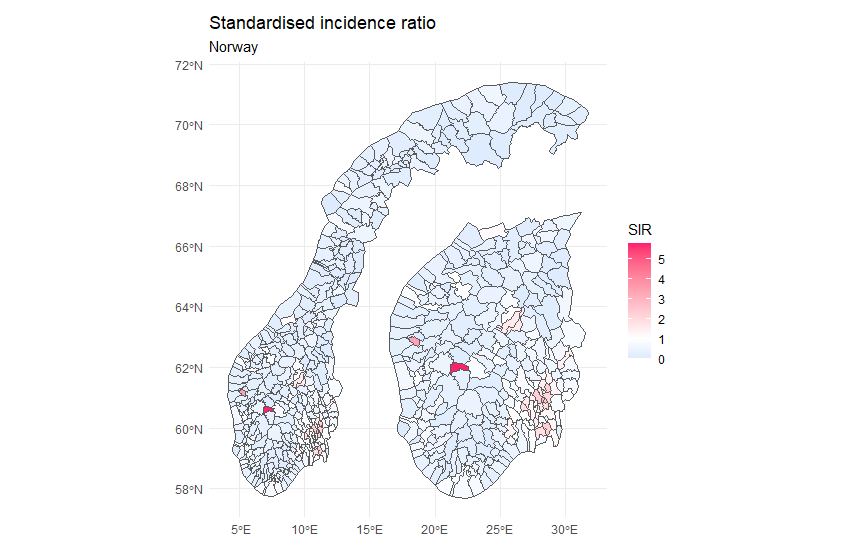
\includegraphics[width = 1.2\textwidth]{sir_norway.png}
  \caption{The standardised incidence ratio for Norway based on the data of the 24th of March 2021}
  \label{sirnorway}
\end{figure}
Because the high numbers from two small municipalities complicate the interpretation of Figure~\ref{sirnorway}, Figure~\ref{sirnorwaylog} shows the SIR on a log10 scale. It is now clearer that the standardized incidence ratio is below 1 in most parts of Norway, but that there is a higher risk in the region around Oslo.
% \begin{figure}[H]
%   \centering
%   \includesvg[width = 1.2\textwidth]{sir_norway_log.svg}
%   \caption{The log10 standardised incidence ratio for Norway based on the data of the 24th of March 2021}
%   \label{sirnorway}
% \end{figure}
\begin{figure}[H]
  \centering
  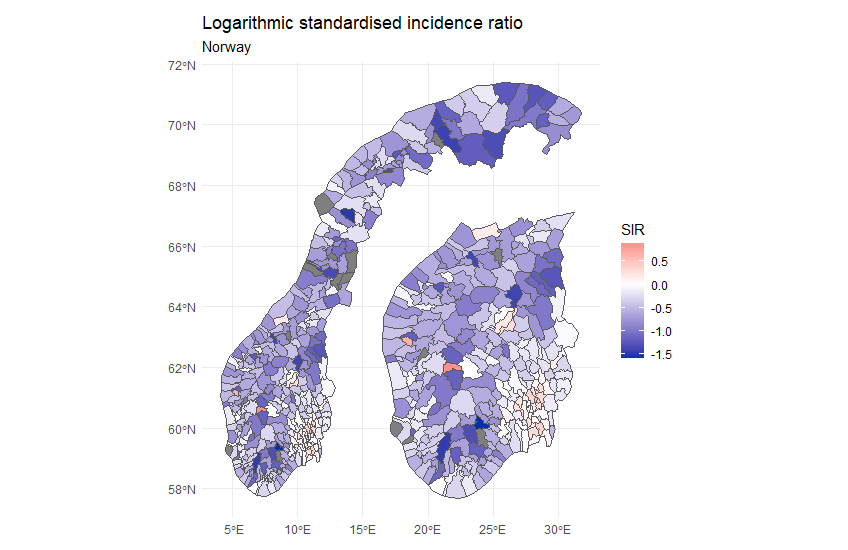
\includegraphics[width = 1.2\textwidth]{sir_norway_log.png}
  \caption{The log10 standardised incidence ratio for Norway based on the data of the 24th of March 2021}
  \label{sirnorwaylog}
\end{figure}
\clearpage
\section{Spatial Models}
After looking at the standardised incidence rates for the countries of interest, the next step is to take a closer look at the current figures for the respective countries. Spatial models are used to try to extract the factors that cause some populations to be at higher risk than other populations. Four different types of models are used for each country:
\begin{itemize}
    \item[1.] The Besarg-Yollie-Mollie Model
    \item[2.] Besags Proper Spatial Model
    \item[3.] The Leroux-Model
    \item[4.] A model without a spatial component
\end{itemize}
All of these models were computed using the INLA \cite{rinla} R package. \\
To specify each type of model, the code shown in Listing~\ref{codeModels} can be used. \\
Four measures are used to compare the models, the DIC, the WAIC, the CPO and the mean absolute error (MAE).\\
For all countries, the models were computed with
\begin{itemize}
    \item[1.] only the demographic variables as covariates
    \item[2.] only the infrastructural variables as covariates
    \item[3.] both, demographic and infrastructural variables, as covariates
    \begin{itemize}
        \item[3.1] Without variable selection
        \item[3.2] With variable selection
    \end{itemize}
\end{itemize}
In addition to specifying what type of spatial model to use, if any, there is also the option of specifying a prior. In this case, a penalised complexity prior is used for the precision $\tau$. For $\tau$, the penalised complexity prior is defined by the parameter $\sigma_0$. The equation~\ref{eq:pcprior} therefore looks like this,
\begin{equation}\label{pcprec}
    \mathbb{P}\left(\sigma > \sigma_0\right)=\alpha.
\end{equation}
The actual expression of the prior is given by
\begin{equation}
    \pi\left(\tau\right)=\frac{\lambda}{2}\tau^{-3/2}\exp\left(-\lambda\tau^{-1/2}\right),\hspace{10pt}\tau>0.
\end{equation}
Here, $\lambda=\frac{-\log\left(\alpha\right)}{U}$ \cite{martins2014penalising}.
For the parameters $\sigma_0$ and $\alpha$, the values 1 and 0.01 were chosen. \\
The models were compared using the mean absolute error. For this, 20\% of the observations were removed from the training and used for testing instead. The predicted number of infections for these municipalities was then compared to the actual numbers.
\\
Finally, due to the amount of covariates, forwards and backwards stepwise variable selection was performed with the intention of obtaining a model that fits the data well and at the same time is relatively easy to interpret. This can be done with the R package \texttt{INLAutils} \cite{inlautils}, as shown in Listing~\ref{codeSelection}. Backwards as well forwards variable selection was performed.\\
A list of all calculated models along with their performance measures is provided in the appendix.
\subsection{Model Selection}
Before the models are computed, however, the distribution that fits the number of cases must first be found. For this, the function \texttt{descdist()} from the \texttt{fitdistrplus} R package is used. The Cullen and Frey graph can be used to give an initial idea of which distributions fit the data, in this case the number of infections, reasonably well depending on the kurtosis and the square of the skewness. \\
The plots for Germany and Norway can be seen in Figure~\ref{cf_germany} and Figure~\ref{cf_norge}.
% \begin{figure}[H]
%     \centering
%     \includesvg[width = 0.8\textwidth]{cf_germany.svg}
%     \caption{The Cullen and Frey graph for Germany}
%     \label{cf_germany}
% \end{figure}
\begin{figure}[H]
    \centering
    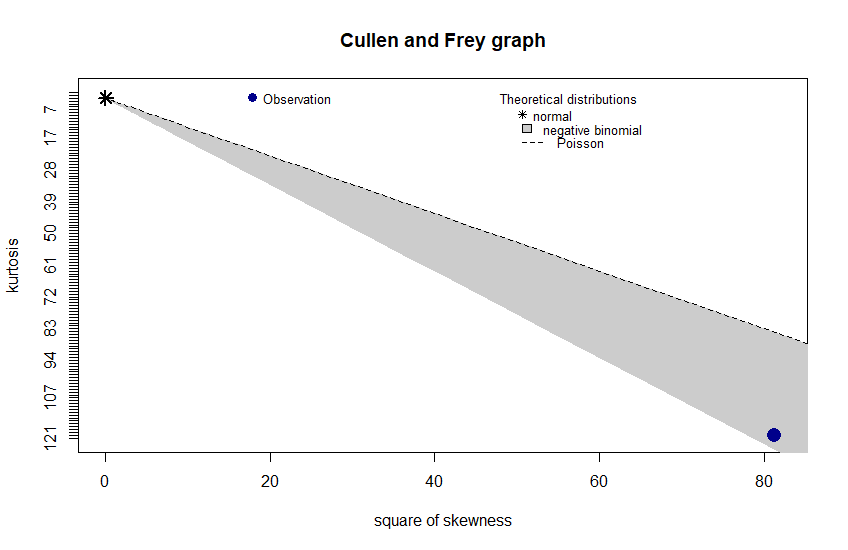
\includegraphics[width = 0.8\textwidth]{cf_germany.png}
    \caption{The Cullen and Frey graph for Germany}
    \label{cf_germany}
\end{figure}
% \begin{figure}[H]
%     \centering
%     \includesvg[width = 0.8\textwidth]{cf_norge.svg}
%     \caption{The Cullen and Frey graph for Norway}
%     \label{cf_norge}
% \end{figure}
\begin{figure}[H]
    \centering
    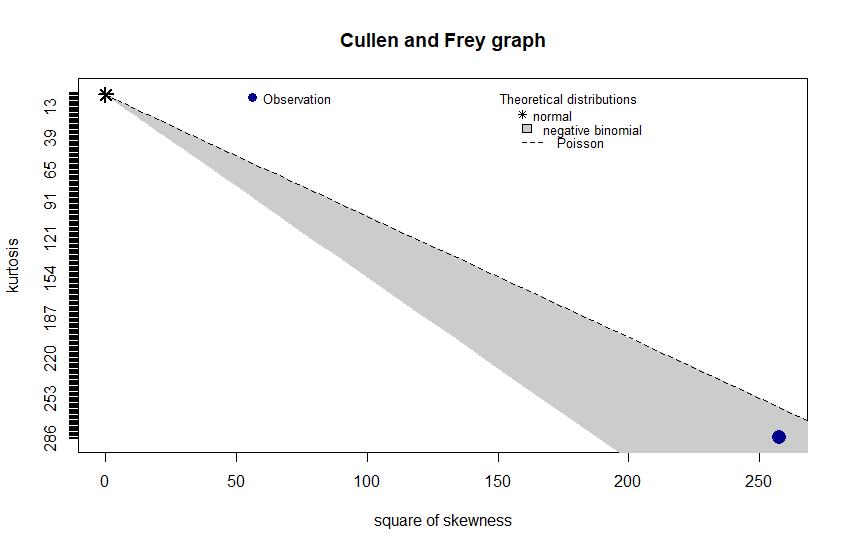
\includegraphics[width = 0.8\textwidth]{cf_norge.png}
    \caption{The Cullen and Frey graph for Norway}
    \label{cf_norge}
\end{figure}
Next, a negative binomial distribution, a normal distribution, and a Poisson distribution are fitted to the data using the maximum likelihood method. The negative binomial fits for both countries can be seen in Figure~\ref{fitNegbinomGermany} and Figure~\ref{fitNegbinomNorway}. The fits for the normal and Poisson distribution for both countries, are shown in the Appendix in Figure~\ref{fitNormalGermany}, Figure~\ref{fitPoissonGermany}, Figure~\ref{fitNormalNorway} and Figure~\ref{fitPoissonNorway}. \\
The QQ-plot for Germany and Norway looks quite similar, as there appears to be a linear relationship between the theoretical quantile and the sample quantiles, up to a certain point where the sample quantiles have a higher value than the theoretical quantiles, indicating that the distribution is right skewed. Since there are many municipalities with relatively few cases and few municipalities with a large number of cases, this is to be expected.
% \begin{figure}[H]
%     \centering
%     \includesvg[width = 0.8\textwidth]{fit_nbinom_germany.svg}
%     \caption{A negative binomial fit to the number of cases in German municipalities}
%     \label{fitNegbinomGermany}
% \end{figure}
\begin{figure}[H]
    \centering
    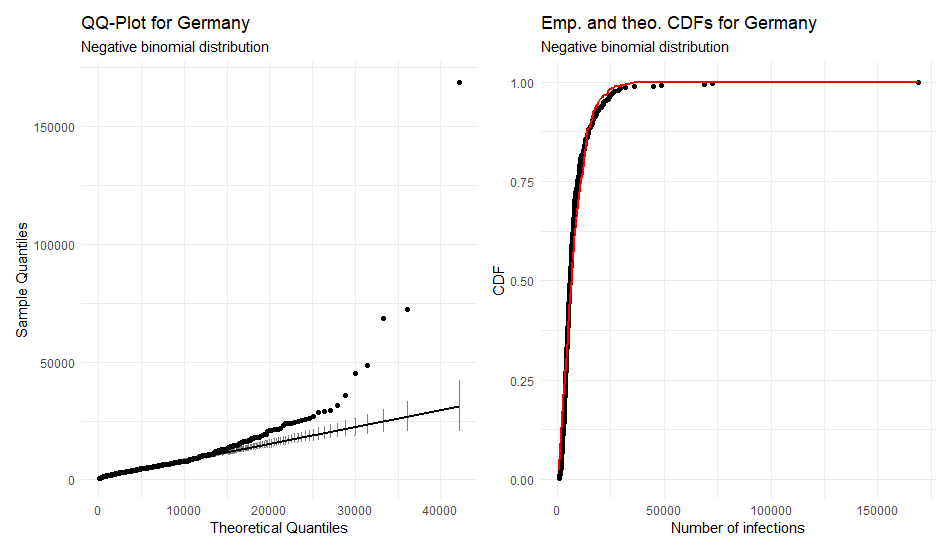
\includegraphics[width = 0.8\textwidth]{fit_nbinom_germany.png}
    \caption{A negative binomial fit to the number of cases in German municipalities}
    \label{fitNegbinomGermany}
\end{figure}
% \begin{figure}[H]
%     \centering
%     \includesvg[width = 0.8\textwidth]{fit_nbinom_norway.svg}
%     \caption{A negative binomial fit to the number of cases in Norwegian municipalities}
%     \label{fitNegbinomNorway}
% \end{figure}
\begin{figure}[H]
    \centering
    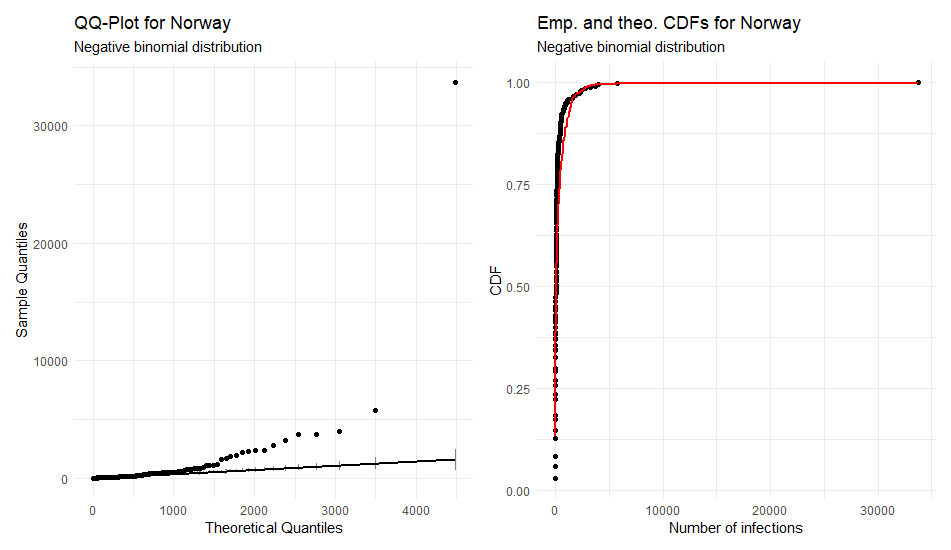
\includegraphics[width = 0.8\textwidth]{fit_nbinom_norway.png}
    \caption{A negative binomial fit to the number of cases in Norwegian municipalities}
    \label{fitNegbinomNorway}
\end{figure}
Lastly, the AIC was calculated for fitting a normal distribution to the data, a Poisson distribution to the data and a negative binomial distribution to the data. The values can be seen in Table~\ref{aic}. Afterwards, the negative binomial distribution was chosen as the distribution of the target variable in both cases. \\
\begin{table}[H] 
\caption{The AIC for different distributions for Germany and Norway \label{aic}}
\begin{tabular}{l l r}
\toprule
\textbf{Country}	& \textbf{Distribution}	& \textbf{AIC} \\
\midrule
Germany & Normal & 8360 \\
Germany & Poisson & 2148100 \\
Germany & Negative Binomial & 7731 \\
Norway & Normal & 6166 \\
Norway & Poisson & 366181 \\
Norway & Negative Binomial & 4086 \\
\bottomrule
\end{tabular}
\end{table} 
The poor fit for the Poisson distribution can be explained by looking at the range of the number of confirmed cases in a given municipality. For Germany, this number ranges from 508 to 137634 (as of March 18, 2021), while for Norway, the number ranges from 0 to 24905 (as of March 20, 2021). This results in a mean and standard deviation for Germany of 6617 and 9014, respectively. For Norway, the values for these metrics are 236 and 1389.
\subsection{Spatial Models for Germany}
First, a look is taken at the spatial models calculated for Germany. These models are based on data from 24 March 2021, when 2.695.037 people in Germany were confirmed infected with Covid-19. The five municipalities with the most infections are shown in Table~\ref{top5germany}.
\begin{table}[H] 
\caption{The municipalities with the most infections as of March 24th 2021. \label{top5germany}}
\begin{tabular}{l r r}
\toprule
\textbf{Municipality}	& \textbf{Population}	& \textbf{Number of infections} \\
\midrule
SK Berlin & 3644826 & 141639   \\     
SK Hamburg & 1841179 & 58661   \\
SK Munich & 1471508 & 57690   \\
SK Cologne & 1085664 & 37592   \\
Region Hannover & 1157624 & 36241   \\
\bottomrule
\end{tabular}
\end{table}
\subsubsection{Demographic Models}\label{sssec:demoGermany}
The model with the best performance based on the demographic variables was a Leroux model computed using the formula in Listing~\ref{codeDemoGermany}. The variables used for this model were the percentages of the vote for the six biggest German political parties. \\
The performance measures of this model and the best-performing BYM2 and Besag proper models are shown in Table~\ref{demoGermany}. 
\begin{table}[H] 
\caption{The performance measures for the best performing demographic model of each type. \label{demoGermany}}
\begin{tabular}{l r r r r}
\toprule
\textbf{Model}	& \textbf{DIC}	& \textbf{WAIC} & \textbf{CPO} & \textbf{MAE}\\
\midrule
Besag  & 4761 & 4712 & -2744 &  225675 \\
BYM2 & 4636 & 4617  & -2723 &  225255\\
Leroux & 4734  & 4749 & -3002 & 221620\\
No Spatial & 5538  & 5539 & -2769 & 223145\\
\bottomrule
\end{tabular}
\end{table}
The summary of the fixed effects is shown in Table~\ref{fixedDemoGermany}. To compute the posterior mean of the coefficients, the code shown in Listing~\ref{codePosteriorMean} can be used. \\
To get the expected value given a marginal function $\pi\left(x\right)$, the expected value of a function $f\left(x\right)$ is calculated, i.e.
\begin{equation*}
    \int f\left(x\right)\pi\left(x\right)dx.
\end{equation*}
To obtain a credibility interval of the fixed effects on the transformed scale, the code in Listing~\ref{codeCredibility} can be used. \\
\begin{table}[H] 
\caption{The fixed effects for the Leroux model. Values are rounded. A $^*$ denotes a significant effect.\label{fixedDemoGermany}}
\begin{tabular}{l r r r r c}
\toprule
\textbf{Variable}	& \textbf{Mean}	& \textbf{exp(mean$_{\hbox{p}}$)} & \textbf{exp(q0025$_{\hbox{p}}$)} & \textbf{exp(q0975$_{\hbox{p}}$)} & \textbf{sig.}\\
\midrule
(Intercept) & -0.08413 & 0.9194 & 0.8892 & 0.9503 &\\
afd & 0.1523 & 1.167& 1.016 & 1.334 &$^*$\\
FDP & -0.08350 & 0.9919& 0.9543 & 1.030 &\\
Gruene & -0.1029 & 0.9046 & 0.7831 & 1.039 &\\
Union & -0.1293 & 0.8817& 0.7486 & 1.031 &\\
SPD & -0.1510 & 0.8606 & 0.7901 & 0.9355 &\\
die\_linke & -0.2077 & 0.8133 & 0.7416 & 0.8898 &\\
\bottomrule
\end{tabular}
\end{table}
The posterior mean of the exponentiated intercept implies a -8.1\% risk rate across Germany with a credibility interval ranging from -11.1\% to -5.0\%. However, this coefficient is not significant. \\
This summary shows that especially people who come from regions where the AfD gets a higher share of the vote have a higher risk of contracting Covid-19. In Figure~\ref{sirgermany}, regions in eastern Germany often had a higher SIR. These are also the regions where the AfD tends to perform better in elections. The connection between the two can be attributed to the fact that the AfD is a right-wing party that openly criticises the measures taken to prevent the spread of the coronavirus. As a result, a large proportion of people who vote for the AfD do not take the measures seriously either and refuse to keep a safe distance or wear a mask in public spaces. \\
Wondreys and Mudde took a look at right-wing parties' responses to the pandemic, pointing out that while these parties were quick to warn about the virus, once cases spiked they criticised the measures taken to contain the spread of the virus. They also noted that right-wing parties supported demonstrations against these measures. However, they also stressed that these parties often rejected the measures proposed by the leading parties because they themselves were part of the opposition, as is the case with the AfD in Germany \cite{wondreys2020victims}.  \\
Farias and Pilati also conducted a study in Brazil to predict social distancing violation intention and past non-compliance during the COVID-19 pandemic, controlling for the effects of intolerance of uncertainty and sociodemographic variables. Their results included that individuals who support right-wing parties are more likely to violate social distancing measures \cite{farias2020violating}. \\
An increase by one standard deviation for the AfD leads to a risk increase of about 16.7\%. No significant effects were observed for all other parties. \\
It is interesting, however, that the party "Die Linke", which is currently the most left-wing party in the German parliament, has the smallest posterior mean. \\
As this was the overall best-performing spatial model for Germany, a look is taken at the posterior means $\pmb{\zeta} = \exp{\left(\xi\right)}$ of the area-specific risks. Since the uncertainty associated with them can also be mapped, the posterior probability $\mathbb{P}\left(\zeta_i > 1|\pmb{y}\right)$ is visualised as well. In Figure~\ref{posteriorGermany}, it can be seen that the relative risk is above 1 for large parts of Germany, except for most of northern Germany and some parts in the south of the country. The posterior probability is highest for parts of North Rhine-Westphalia, home to Germany's most populous metropolitan area, the Ruhr area, and for Saxony and Thuringia, both political strongholds of the AfD. The higher numbers in Bavaria can be explained by the large common borders with Austria and the Czech Republic, two countries that were more affected by the pandemic. Many people cross these borders because of tourism and many guest workers come from the Czech Republic to work on agricultural land in Bavaria, which resulted in several Covid-19 outbreak events.
\begin{figure}[H]
    \centering
    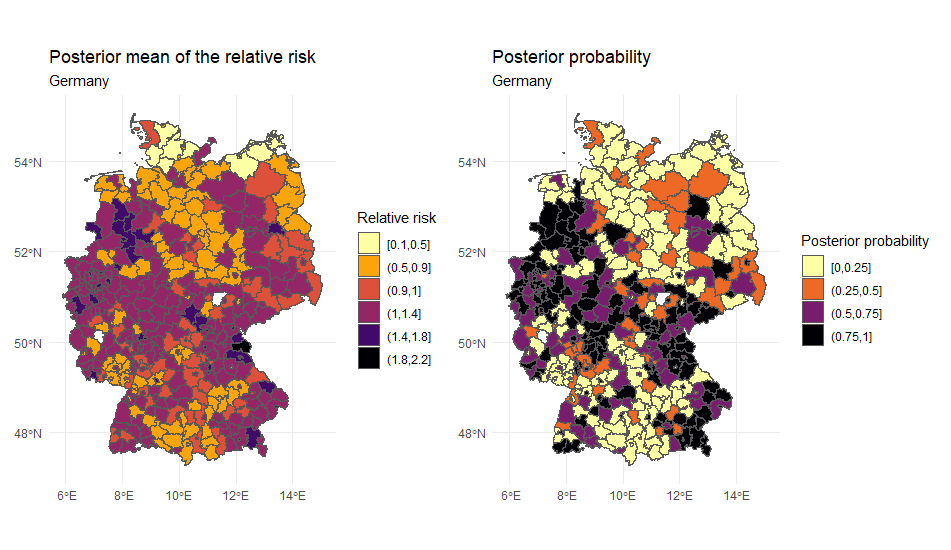
\includegraphics[width = \textwidth]{posterior_germany.png}
    \caption{Posterior mean of the area-specific risk and the posterior probability.}
    \label{posteriorGermany}
\end{figure}
% \begin{figure}[H]
%     \centering
%     \includesvg[width = textwidth]{posterior_germany.svg}
%     \caption{A negative binomial fit to the number of cases in Norwegian municipalities}
%     \label{nb_norge}
% \end{figure}
Compared to the standardised incidence rate in Germany, shown in Figure~\ref{sirgermany}, it can be seen that the parts of Germany with the lowest SIR, Northern Germany, are also the parts of Germany with the lowest relative risk. Saxony had the highest SIR and also has an increased relative risk. Most parts of Germany that had an SIR of around 1 have a relative risk between 1 and 1.4.
\subsubsection{Infrastructure Models}\label{sssec:infraGermany}
When it comes to the models based on the infrastructural variables, a model without any spatial component performed the best. It was computed using formula in Listing~\ref{codeInfraGermany}. \\
The performance measures of this model and the best-performing other models are shown in Table~\ref{infraGermany}
\begin{table}[H] 
\caption{The performance measures for the best performing infrastructure model of each type. \label{infraGermany}}
\begin{tabular}{l r r r r}
\toprule
\textbf{Model}	& \textbf{DIC}	& \textbf{WAIC} & \textbf{CPO} & \textbf{MAE}\\
\midrule
Besag & 4753 & 4708 & -2772 & 225502\\
BYM2 & 4674 & 4664 & -2767 & 223208\\
Leroux & 4767 & 4787 & -3278 & 200001\\
No Spatial & 5655 & 5654 & -2847 & 189664\\
\bottomrule
\end{tabular}
\end{table}
The values of the covariates are shown in Table~\ref{fixedInfraGermany}.
\begin{table}[H] 
\caption{The fixed effects for the model without a spatial component. Values are rounded. A $^*$ denotes a significant effect.\label{fixedInfraGermany}}
\begin{tabular}{l r r r r c}
\toprule
\textbf{Variable}	& \textbf{Mean}	& \textbf{exp(mean$_{\hbox{p}}$)} & \textbf{exp(q0025$_{\hbox{p}}$)} & \textbf{exp(q0975$_{\hbox{p}}$)} & \textbf{sig.}\\
\midrule
(Intercept) & -0.02831 & 0.9723 & 0.9373 & 1.009 &\\
bakeries & 0.5143 & 1.683 & 1.351 & 2.074 &$^*$\\
pop\_dens & 0.1089 & 1.116 & 1.049 & 1.187 & $^*$\\
place\_of\_ & \multirow{2}{*}{0.09044} & \multirow{2}{*}{1.095} & \multirow{2}{*}{1.033} & \multirow{2}{*}{1.160} &\multirow{2}{*}{$^*$}\\
worship &  \\
higher\_ & \multirow{2}{*}{0.008236} & \multirow{2}{*}{1.009} & \multirow{2}{*}{0.9536} & \multirow{2}{*}{1.069} &\\
education \\
nursing\_home & 0.006448 & 1.007 & 0.9602 & 1.057 &\\
entertainment & -0.01045 & 0.9936 & 0.8311 & 1.180 &\\
platform & -0.01408 & 0.9868 & 0.9147 & 1.064 &\\
aerodrome & -0.01525 & 0.9850 & 0.9541 & 1.020 &\\
sport & -0.06345 & 0.9401 & 0.8371 & 1.053 \\
schools & -0.08823 & 0.9178 & 0.7980 & 1.051 &\\
retail & -0.1295 & 0.8792 & 0.8128 & 0.9524 &\\
kindergarten & -0.1346 & 0.8805 & 0.6907 & 0.9524 &\\
hairdresser & -0.1401 & 0.8752 & 0.6925 & 1.092 &\\
restaurant & -0.1757 & 0.8425 & 0.6995 & 1.008 &\\
\bottomrule
\end{tabular}
\end{table}
Findings from these results are that bakeries, places of worship and population density increase the risk of infection. For bakeries, an increase of 1 standard deviation leads to a risk increase of 68.3\%. Bakeries are relatively widespread in Germany and many people go there several times a week to get fresh bread or other baked goods. When many people congregate in bakeries, viruses can spread more easily. \\
A 1 standard deviation increase in population density leads to an 11.6\% increase in relative risk, which should not be too surprising since in communities with higher population density, people come into contact with more people, which in turn helps the virus move from host to host. \\
Finally, places of worship were not closed for a long time in Germany due to freedom of religion and therefore people gathered in churches, mosques and the like. A 1 standard deviation increase in these places of worship therefore leads to a 9.5\% increase in the risk of contracting Covid-19. \\
Yezli and Khan's paper argues for the closure of these places of worshipon the grounds that they pose a risk of transmitting COVID-19 to potentially large numbers of people through a single case. Gatherings at these places often involve dense mixing of many people in a confined space, sometimes for long periods of time \cite{yezli2020covid}.
\subsubsection{Combined Models}
Finally, models are considered that include both the infrastructural and demographic covariates. Due to the amount of variables, all models run are based on variable selection. \\
The best performing model was again a model with no spatial component, computed with the formula shown in Listing~\ref{codeBothGermany}. \\
The performance measures of the computed models are shown in Table~\ref{allGermany}.
\begin{table}[H] 
\caption{The performance measures for the best performing demographic + infrastructure model of each type. \label{allGermany}}
\begin{tabular}{l r r r r}
\toprule
\textbf{Model}	& \textbf{DIC}	& \textbf{WAIC} & \textbf{CPO} & \textbf{MAE}\\
\midrule
Besag&  4806 & 4739 & -2711 & 362281\\
BYM2 & 4665 & 4651 & -2704 & 350752\\
Leroux & 5020 & 5022 & -2882 & 280649 \\
No Spatial & 5423 & 5423 & -2721 & 273879 \\
\bottomrule
\end{tabular}
\end{table}
The fixed effects are shown in Table~\ref{fixedAllGermany}.

\begin{table}[H] 
\caption{The fixed effects for the model without a spatial component. Values are rounded. A $^*$ denotes a significant effect.\label{fixedAllGermany}}
\begin{tabular}{l r r r r c}
\toprule
\textbf{Variable}	& \textbf{Mean}	& \textbf{exp(mean$_{\hbox{p}}$)} & \textbf{exp(q0025$_{\hbox{p}}$)} & \textbf{exp(q0975$_{\hbox{p}}$)} & \textbf{sig.}\\
\midrule
(Intercept) & -0.0712 & 0.9314 & 0.9047 & 0.9589 \\
unemployed\_ & \multirow{2}{*}{0.6614} & \multirow{2}{*}{1.954} & \multirow{2}{*}{1.506} & \multirow{2}{*}{2.492} & \multirow{2}{*}{$^*$}\\
foreigners \\
afd & 0.2023  & 1.225 & 1.147 & 1.308 & $^*$\\
pop\_dens & 0.1245 & 1.133 & 1.072 & 1.197 & $^*$\\
shops & 0.1234 & 1.143 & 0.8593 & 1.489 \\
schools & 0.1177 &1.127 & 1.002 & 1.264 & $^*$\\
kindergarten & 0.07769 & 1.085 & 0.9052 & 1.292 \\
sex & 0.06440 &1.067 & 1.031 & 1.103 & $^*$\\
higher\_ & \multirow{2}{*}{0.06279} & \multirow{2}{*}{1.065} & \multirow{2}{*}{1.021} & \multirow{2}{*}{1.111} & \multirow{2}{*}{$^*$} \\
education & \\
entertainment & 0.04197 & 1.046 & 0.9073 & 1.120 \\
clinic & 0.03603&  1.037 & 0.9609 & 1.120 \\
sport & 0.03435& 1.036 & 0.9478 & 1.130 \\
platform & 0.01969 &  1.020 & 0.9581 & 1.086 \\
log & \multirow{2}{*}{0.01426} & \multirow{2}{*}{1.015} & \multirow{2}{*}{0.9776} & \multirow{2}{*}{1.051} \\
income\_total\\
place\_of\_ & \multirow{2}{*}{0.01288} & \multirow{2}{*}{1.013} & \multirow{2}{*}{0.9646} & \multirow{2}{*}{1.064} \\
worship\\
protection\_ & \multirow{2}{*}{0.01186} & \multirow{2}{*}{1.015} & \multirow{2}{*}{0.8636} & \multirow{2}{*}{1.185} \\
seekers\\
aerodrome & 0.0004896 & 1.006 & 0.9766 & 1.027 \\
nursing\_home & -0.002786 & 0.9974 & 0.9636 & 1.032 \\ 
FDP & -0.01863 & 0.9817 & 0.9464 & 1.018 \\
retail & -0.01983 & 0.9809 & 0.9179 & 1.048 \\
log & \multirow{2}{*}{-0.03577} & \multirow{2}{*}{0.9650} & \multirow{2}{*}{0.9362} & \multirow{2}{*}{0.9940} \\
trade\_tax \\
log & \multirow{2}{*}{-0.4560} & \multirow{2}{*}{0.9557} & \multirow{2}{*}{0.9152} & \multirow{2}{*}{0.9973} \\
income\_tax \\
welfare\_ & \multirow{2}{*}{-0.07744} & \multirow{2}{*}{0.9277} & \multirow{2}{*}{0.8096} & \multirow{2}{*}{1.058} \\
recipients &  \\
bakeries & -0.07973 & 0.9273 & 0.7711 & 1.105 \\
office & -0.1081 & 0.8985 & 0.8175 & 0.9855 \\
SPD & -0.1100 & 0.8959 & 0.8668 & 0.9259 \\
die\_linke & -0.1627 & 0.8502 & 0.8043 & 0.8980 \\
restaurant & -0.1939 & 0.8262 & 0.7092 & 0.9576 \\
Gruene & -0.1943 & 0.8239 & 0.7726 & 0.8775 \\
unemployed\_ & \multirow{2}{*}{-0.6720} & \multirow{2}{*}{0.5163} & \multirow{2}{*}{0.3827} & \multirow{2}{*}{0.6818} \\
total & \\
\bottomrule
\end{tabular}
\end{table}
According to this model, the three biggest driving factors for the number of infections are the amount of unemployed foreigners, the share of the vote for the AfD and the population density. The influence of the AfD was already discussed in Section~\ref{sssec:demoGermany}, only in this case an increase of 1 standard deviation leads to a risk increase of 22.5\%. In Section~\ref{sssec:infraGermany} population density was discussed. Here, a 1 standard deviation increase leads to a 13.3\% increase in relative risk. For unemployed foreigners, a 1 standard deviation increase leads to a 95.4\% increase in risk. \\
Other factors that positively influence the risk of infection are the number of schools, the proportion of women in the population and the number of higher educational institutions. A 1 standard deviation increase in the number of schools leads to a 12.7\% increase in risk, which could be an indicator that schools should remain closed because so many children from different households meet there, providing a good place for a virus to spread. Schools in Germany actually closed relatively late, and did reopen at the beginning of 2021.\\
A 1 standard deviation increase in the proportion of women leads to a 6.7\% increase in risk and for higher education buildings a 1 standard deviation increase leads to a 6.5\% increase in risk. 
\subsection{Spatial Models for Norway}
Next, the same types of models are evaluated for Norway. These models are based on data from 24 March 2021, when 87537 people in Norway were confirmed infected with Covid-19. The five municipalities with the most infections are shown in Table~\ref{top5norway}.
\begin{table}[H] 
\caption{The municipalities with the most infections as of March 24th 2021. \label{top5norway}}
\begin{tabular}{l r r}
\toprule
\textbf{Municipality}	& \textbf{Population}	& \textbf{Number of infections} \\
\midrule
Oslo & 693494 & 26151 \\
Bergen & 283929 & 4738 \\
Drammen & 101386 & 3149 \\
Bærum & 127731 & 2834 \\
Lillestrøm & 85983 & 2779 \\
\bottomrule
\end{tabular}
\end{table}
\subsubsection{Demographic Models}\label{sssec:demoNorway}
The best demographic model was a model without any spatial component calculated using the formula shown in Listing~\ref{codeDemoNorway}. \\
The performance measures for all four models are shown in Table~\ref{demoNorway}. It is noticeable that the mean error in Norway is significantly smaller, suggesting that the models for Germany have greatly overestimated or underestimated the number of infections.
\begin{table}[H] 
\caption{The performance measures for the best performing demographic model of each type. \label{demoNorway}}
\begin{tabular}{l r r r r}
\toprule
\textbf{Model}	& \textbf{DIC}	& \textbf{WAIC} & \textbf{CPO} & \textbf{MAE}\\
\midrule
Besag  & 2396 & 2403 & -4369 & 10149 \\
BYM2 & 2224 & 2202 & -6793 & 10002\\
Leroux & 2225  & 2192 & -6810 & 8460\\
No Spatial & 2696  & 2702 & -1376 & 7710\\
\bottomrule
\end{tabular}
\end{table}
All other performance measures for these models are also lower than for the models computed for Germany. \\
The effects of the covariates are shown in Table~\ref{fixedDemoNorway}.
\begin{table}[H] 
\caption{The fixed effects for the model without a spatial component. Values are rounded. A $^*$ denotes a significant effect.\label{fixedDemoNorway}}
\begin{tabular}{l r r r r c}
\toprule
\textbf{Variable}	& \textbf{Mean}	& \textbf{exp(mean$_{\hbox{p}}$)} & \textbf{exp(q0025$_{\hbox{p}}$)} & \textbf{exp(q0975$_{\hbox{p}}$)} & \textbf{sig.}\\
\midrule
(Intercept) & -0.7857 & 0.4563 & 0.4151 & 0.5015 & \\
unemp\_total & 0.3785 & 1.466 & 1.229 & 1.738 & $^*$\\
unemp\_immg & 0.1284 & 1.141 & 0.9752 & 1.334 & \\
\bottomrule
\end{tabular}
\end{table}
The only significant influence on the number of infections is the total number of unemployed people in a municipality. A 1 standard deviation increase in total unemployment leads to a 46.6\% increase in the risk. A possible explanation for this could be that the unemployed spend less time at home and instead move around more and thus have more contact with people, but this should be taken with a grain of salt.
\subsubsection{Infrastructure Models}
For the models based on the infrastructure variables, the best predictive performance was again observed for a model without a spatial component. The formula is shown in Listing~\ref{codeInfraNorway}. \\
The performance measure for the models is shown in Table~\ref{infraNorway}.
\begin{table}[H] 
\caption{The performance measures for the best performing infrastructure model of each type. \label{infraNorway}}
\begin{tabular}{l r r r r}
\toprule
\textbf{Model}	& \textbf{DIC}	& \textbf{WAIC} & \textbf{CPO} & \textbf{MAE} \\
\midrule
Besag  & 2326 & 2335 & -8405 & 11694 \\
BYM2 & 2218 & 2187 & -6532 & 11866\\
Leroux &  2230 & 2167 & -7128 & 12943\\
No Spatial & 2711 & 2716 & -1594 & 11094 \\
\bottomrule
\end{tabular}
\end{table}
The effect of the covariates are shown in Table~\ref{fixedInfraNorway}.
\begin{table}[H] 
\caption{The fixed effects for the model with no spatial component. Values are rounded. A $^*$ denotes a significant effect.\label{fixedInfraNorway}}
\begin{tabular}{l r r r r c}
\toprule
\textbf{Variable}	& \textbf{Mean}	& \textbf{exp(mean$_{\hbox{p}}$)} & \textbf{exp(q0025$_{\hbox{p}}$)} & \textbf{exp(q0975$_{\hbox{p}}$)} & \textbf{sig.}\\
\midrule
(Intercept) & -0.7717 & 0.4628 & 0.4204 & 0.5094 &\\
pop\_dens & 0.5154 & 1.688 & 1.318 & 2.181 & $^*$ \\
schools & 0.4272 & 1.577 & 0.9724 & 2.458 & \\
kindergarten & 0.2583 & 1.317 & 0.9140 & 1.868 \\
nursing\_home & 0.03801 & 1.040 & 0.9542 & 1.152 \\
place\_of\_ & \multirow{2}{*}{-0.08318} & \multirow{2}{*}{0.9324} & \multirow{2}{*}{0.0.6746} & \multirow{2}{*}{1.270} & \multirow{2}{*}{}\\
worship\\
office &-0.1311 & 0.8819 & 0.7206 & 1.082\\
restaurant & -0.2211 & 0.8448 & 0.4220 & 1.501 & \\
shops & -0.5423 &0.6579 & 0.2214 & 1.541 & \\
\bottomrule
\end{tabular}
\end{table}
Again, only one significant effect was observed, the population density. A 1 standard deviation increase leads to a risk increase of 68,8\%. The effect of the population density  has already been discussed in Section~\ref{sssec:infraGermany}
\subsubsection{Combined Models}
For the models containing variables related to the demographic of Norway and the infrastructure, again a Besag model performed the best. Its formula can be seen in Listing~\ref{codeBothNorway}. \\
The performance measures for the models are shown in Table~\ref{bothNorway}
\begin{table}[H] 
\caption{The performance measures for the best performing demographic + infrastructure model of each type. \label{bothNorway}}
\begin{tabular}{l r r r r}
\toprule
\textbf{Model}	& \textbf{DIC}	& \textbf{WAIC} & \textbf{CPO} & \textbf{MAE} \\
\midrule
Besag  & 2395 & 2402 & -5000 & 13111 \\
BYM2 & 2215 & 2184 & -6406 & 13932\\
Leroux &  2229 & 2193 & -7677 & 14841\\
No Spatial & 2676 & 2682 & -1532 & 13479 \\
\bottomrule
\end{tabular}
\end{table}
The fixed effects are shown in Table~\ref{fixedAllNorway}.
\begin{table}[H] 
\caption{The fixed effects for the Besag model. Values are rounded. A $^*$ denotes a significant effect.\label{fixedAllNorway}}
\begin{tabular}{l r r r r c}
\toprule
\textbf{Variable}	& \textbf{Mean}	& \textbf{exp(mean$_{\hbox{p}}$)} & \textbf{exp(q0025$_{\hbox{p}}$)} & \textbf{exp(q0975$_{\hbox{p}}$)} & \textbf{sig.}\\
\midrule
(Intercept) & -1.055 & 0.3534 & 0.2464 & 0.4885 &\\
construction\_ & \multirow{2}{*}{0.1905} & \multirow{2}{*}{1.239} & \multirow{2}{*}{0.7927} & \multirow{2}{*}{1.853}  \\
pt\_work \\
clinic & 0.1735 & 1.252 & 0.6368 & 2.226 \\
pop\_dens & 0.1717 & 1.194 & 0.9701 & 1.456 \\
unemp\_tot & 0.1583 & 1.173 & 1.058 & 1.297 & $^*$\\
schools & 0.1068 & 1.127 & 0.8121 & 1.529 &\\
sex & 0.04749 & 1.050 & 0.9453 & 1.163 \\
restaurant & 0.03536 & 1.085 & 0.5718 & 1.873\\
higher\_& \multirow{2}{*}{-0.06041} & \multirow{2}{*}{0.9434} & \multirow{2}{*}{0.8270} & \multirow{2}{*}{1.070}\\
education\\
median\_age & -0.1117 & 0.8957 & 0.8034 & 0.9950 & \\
workers\_ft\_ & \multirow{2}{*}{-0.5226} & \multirow{2}{*}{0.6396} & \multirow{2}{*}{0.2753} & \multirow{2}{*}{1.264} \\
work\\
\bottomrule
\end{tabular}
\end{table}
Again, only 1 significant effect was found, again the total number of unemployed people. This time, a 1 standard deviation increase leads to a risk increase of 17.3\%, which seems to be a more reasonable figure than the one from the demographic model in Section~\ref{sssec:demoNorway}. \\
Looking at the posterior mean relative risk, it can be seen that the region in and around the capital Oslo is most at risk, as the posterior mean of the relative risk can be as high as 6, with a posterior probability between 0.75 and 1. In addition, some municipalities around Bergen and Ulvik are also more at risk, with a relative risk of up to 3.4 and a posterior probability between 0.75 and 1. \\
The risk seems to be lowest in the parts north of Trondheim and south of Bodø, where the relative risk is mostly below 1. For many municipalities in Troms og Finnmark, the northernmost part of Norway, the posterior mean is also below 1, but for a few regions it is above 1 with posterior probabilities between 0.5 and 0.75 and 0.75-1.
\begin{figure}[H]
    \centering
    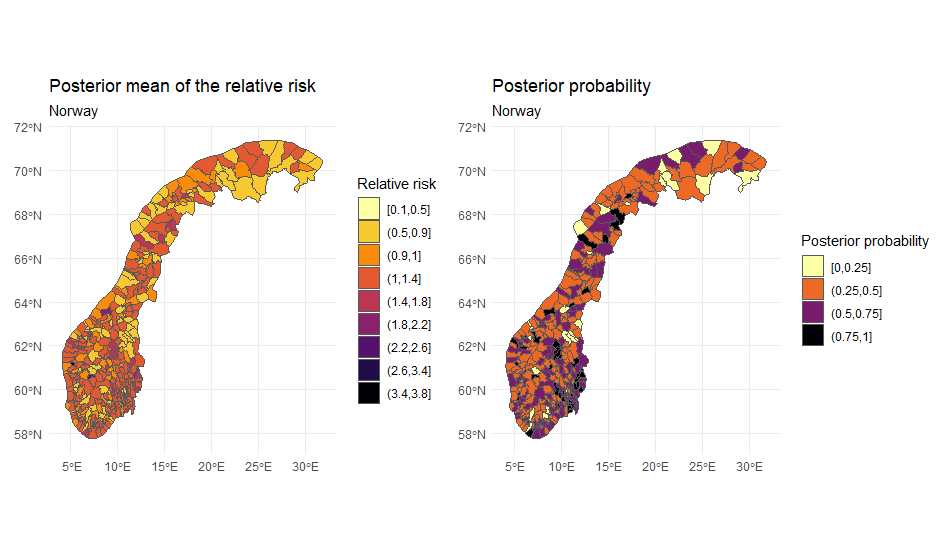
\includegraphics[width = \textwidth]{posterior_norway.png}
    \caption{Posterior mean of the area-specific risk and the posterior probability.}
    \label{posteriorNorway}
\end{figure}
% \begin{figure}[H]
%     \centering
%     \includesvg[width = \textwidth]{posterior_norway.svg}
%     \caption{Posterior mean of the area-specific risk and the posterior probability.}
%     \label{posteriorNorway}
% \end{figure}
For better interpretability, the logarithmic posterior mean is shown in Figure~\ref{posteriorNorwayLog}.
\begin{figure}[H]
    \centering
    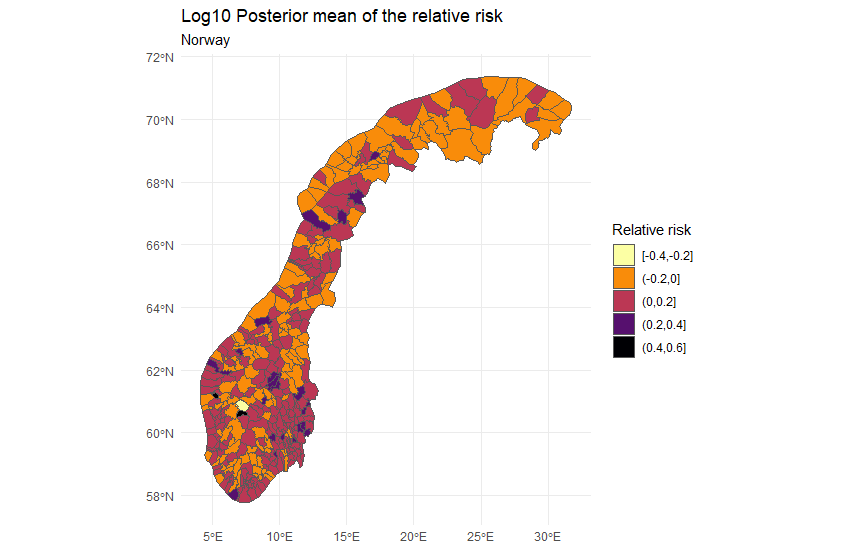
\includegraphics[width = \textwidth]{posterior_norway_log.png}
    \caption{Logarithmic posterior mean of the area-specific risk.}
    \label{posteriorNorwayLog}
\end{figure}
% \begin{figure}[H]
%     \centering
%     \includesvg[width = \textwidth]{posterior_norway_log.svg}
%     \caption{Logarithmic posterior mean of the area-specific risk.}
%     \label{posteriorNorwayLog}
% \end{figure}
Comparing the log relative risk with the log standardised incidence ratio in Figure~\ref{sirnorwaylog}, these two are quite similar. For most parts of Norway, the risk is at or below 0, while there is an increased risk in the Oslo region. However, there are a few municipalities that have a log-standardised incidence ratio of about 0, but a higher log-relative risk than this. Most of these are located in southern Norway, but a few are scattered throughout the rest of the country.
\clearpage
\subsection{Choice of Prior Sensitivity}
As can be seen in equation~\ref{pcprec}, there is flexibility when it comes to choosing the values for the standard deviation $\sigma_0$ as well as the probability $\alpha$. Therefore, an upper bound for the standard deviation can be chosen as well as the weight placed on this "tail event", describing how informative the resulting prior is. In the following, an assessment is made of how the performance of a Besag model, a BYM2 model and a Leroux model changes when playing around with these two values.
\subsubsection{Changing the Value for the Standard Deviation}
By allowing the precision to be greater, the variance is forced to be smaller. Hence, choosing a higher value for the precision leads to lower values for the DIC, WAIC and CPO, as can be seen in Figure~\ref{comparison_norway_1} and Figure~\ref{comparison_norway_2}. While this indicates a better fit to the training data, Figure~\ref{comparison_norway_2} also shows that the MAE increases when a higher value for $U=\sigma_0$ is chosen, as the models overfit on the training data and therefore make worse predictions. \\
The corresponding figures for Germany are shown in Figure~\ref{comparison_germany_1} and Figure~\ref{comparison_germany_2} in the Appendix.
\begin{figure}[H]
    \centering
    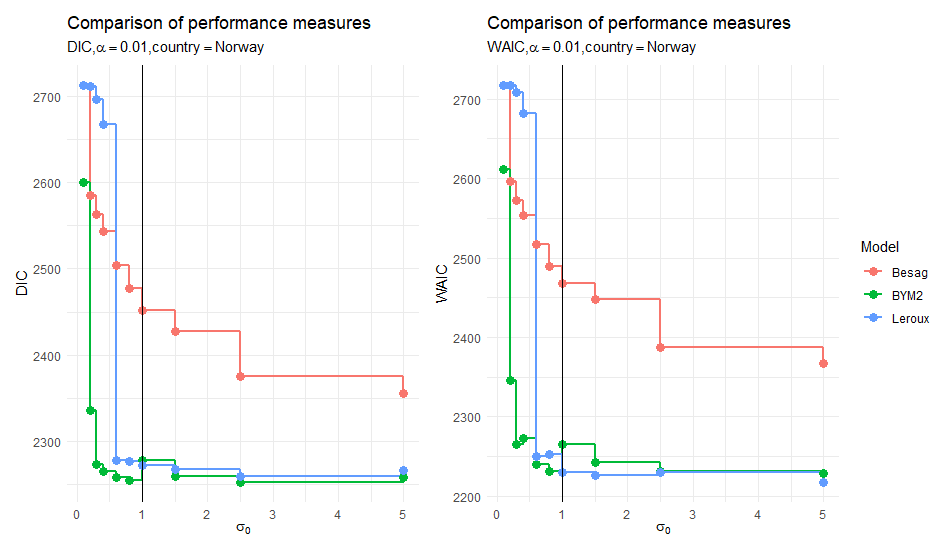
\includegraphics[width = \textwidth]{comparison_1_norway.png}
    \caption{Value of the DIC and WAIC when changing the value for $\sigma_0$. The black line highlights the values for $\sigma_0$ = 1.}
    \label{comparison_norway_1}
\end{figure}
% \begin{figure}[H]
%     \centering
%     \includesvg[width = \textwidth]{comparison_1_norway.svg}
%     \caption{Value of the DIC and WAIC when changing the value for $\sigma_0$. The black line highlights the values for $\sigma_0$ = 1.}
%     \label{comparison_norway_1}
% \end{figure}
\begin{figure}[H]
    \centering
    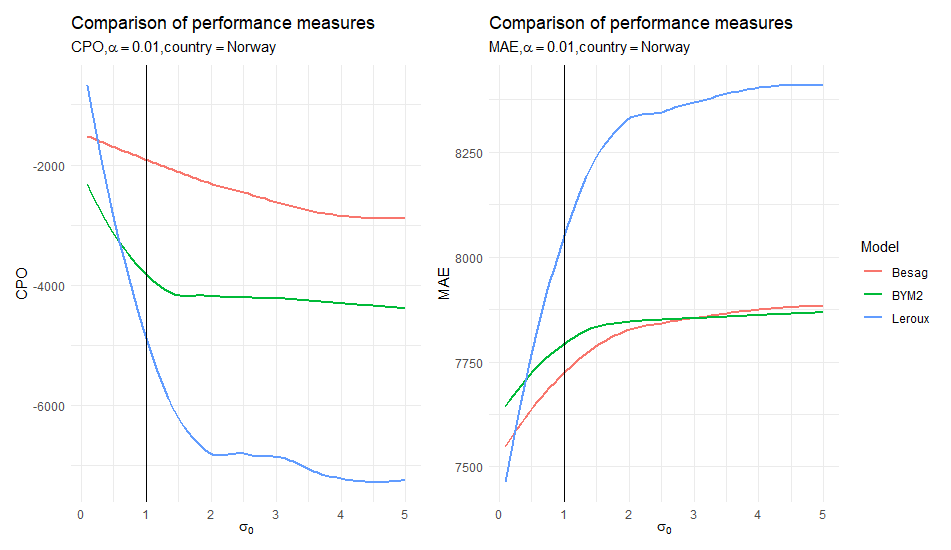
\includegraphics[width = \textwidth]{comparison_2_norway.png}
    \caption{Value of the CPO and MAE when changing the value for $\sigma_0$. The black line highlights the values for $\sigma_0$ = 1.}
    \label{comparison_norway_2}
\end{figure}
% \begin{figure}[H]
%     \centering
%     \includesvg[width = \textwidth]{comparison_2_norway.svg}
%     \caption{Value of the CPO and MAE when changing the value for $\sigma_0$. The black line highlights the values for $\sigma_0$ = 1.}
%     \label{comparison_norway_2}
% \end{figure}

\subsubsection{Changing the Value for the Probability}
By allowing the probability to be greater, the certainty with which the accuracy is 1 becomes less and it could therefore actually be greater than 1. Therefore, a trend similar to that seen in Figure~\ref{comparison_norway_1} and Figure~\ref{comparison_norway_2} can be seen. Choosing a higher value for the probability leads to lower values for the DIC, WAIC and CPO and a higher value for MAE, as can be seen in Figure~\ref{comparison_norway_3} and Figure~\ref{comparison_norway_4}. \\
The corresponding figures for Germany are shown in Figure~\ref{comparison_germany_3} and Figure~\ref{comparison_germany_4} in the Appendix.
\begin{figure}[H]
    \centering
    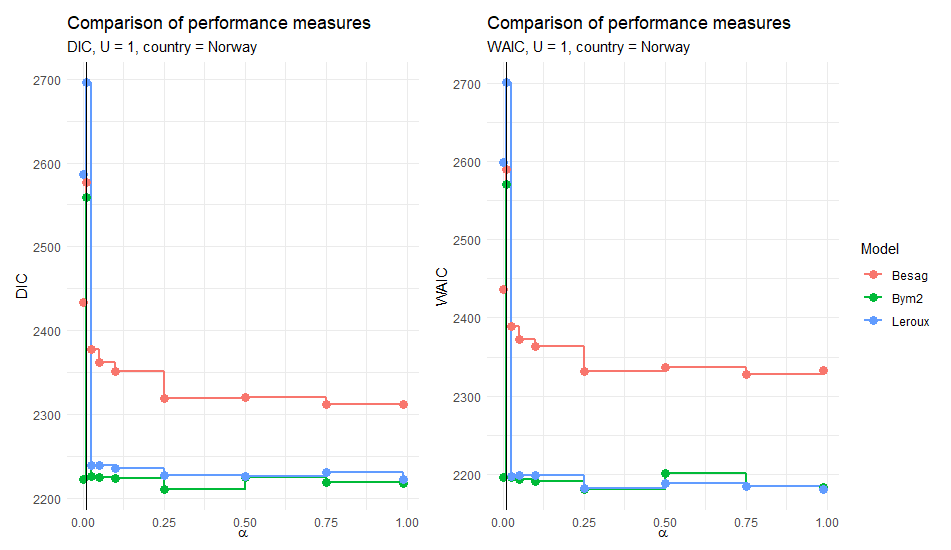
\includegraphics[width = \textwidth]{comparison_3_norway.png}
    \caption{Value of the DIC and WAIC when changing the value for $\alpha$. The black line highlights the values for $\alpha$ = 0.01.}
    \label{comparison_norway_3}
\end{figure}
% \begin{figure}[H]
%     \centering
%     \includesvg[width = \textwidth]{comparison_3_norway.svg}
%     \caption{Value of the DIC and WAIC when changing the value for $\alpha$. The black line highlights the values for $\alpha$ = 0.01.}
%     \label{comparison_norway_3}
% \end{figure}
\begin{figure}[H]
    \centering
    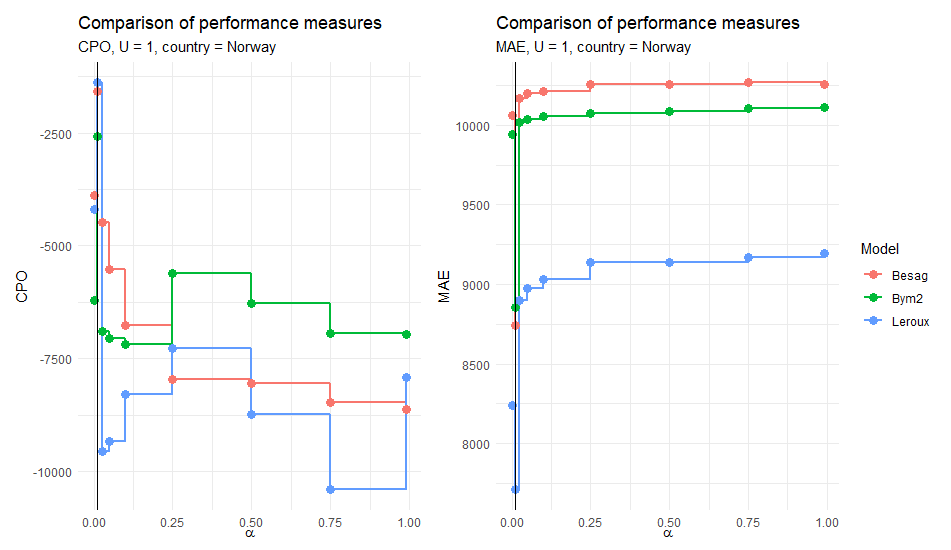
\includegraphics[width = \textwidth]{comparison_4_norway.png}
    \caption{Value of the CPO and MAE when changing the value for $\alpha$. The black line highlights the values for $\alpha$ = 0.01.}
    \label{comparison_norway_4}
\end{figure}
% \begin{figure}[H]
%     \centering
%     \includesvg[width = \textwidth]{comparison_4_norway.svg}
%     \caption{Value of the CPO and MAE when changing the value for $\alpha$. The black line highlights the values for $\alpha$ = 0.01.}
%     \label{comparison_norway_4}
% \end{figure}

\clearpage
\section{Spatio-Temporal Models}
\subsection{Spatio-Temporal Models for Germany}
\subsection{Spatio-Temporal Models for Norway}
\clearpage
\section{Predictive Models}
\subsection{Predictive Models for Germany}
\subsection{Predictive Models for Norway}